\documentclass[12pt]{mitthesis} 
\usepackage[pdftex]{graphicx}
\usepackage{kylesthesis}
\begin{document}

\tableofcontents
\clearpage

\subsubsection*{NOTES}
\clearpage

\chapter{Collisional excitation of molecular triplet states by atomic
  metastables}

\section{Introduction}


Although molecular triplet states are hard to populate optically, they
are easily generated in electronic-energy exchanging collisions.  In
fact, this property is one of the primary resons for studying triplets
in the first place.  We should be able to generate large numbers of
triplet molecules by first creating large numbers of metastable atoms,
and then letting collisions do the work.

The process of mercury photosentization is well-known in organic
chemistry \cite{brown89, brown88, crabtree92, cvetanovic64,
  phillips74, strausz70}.  The common technique is to place mercury
and reactants in a heated reaction vessel, and irradiate with 257 nm
light from a mercury resonance lamp \cite{brown87}.

The first experimental detection of acetylene triplet states was
accomplished using the process of mercury photosensitization.  Later,
Kanamori and coworkers have used mercury photosensitization to study
the \emph{cis}-$T_2$ $\leftarrow$ \emph{cis}-$T_1$ absorption spectrum
of acetylene \cite{kanamori07}.

The main drawback to using a traditional mercury photosensitization
technique with acetylene is polymer formation.  This process is well
known to photochemists \cite{shida58, leroy44}, and to any unfortunate
spectroscopists who have used the technique.  Another problem is the
complicated dynamics of radiation trapping and energy pooling in
mercury following 254 nm resonance excitation \cite{menningen00,
  herd05, majetich89, majetich91}.

The rate of polymer formation could be kept to a minimum if the number
density of mercury atoms could be carefully controlled.  In addition,
it would be nice if the particular atomic metastable state could be
selected based on the desired electronic energy.  In addition, we
would like to carry out experiments in a molecular beam, so that
rotational and vibrational cooling could concentrate the population of
triplet molecules to a relatively small number of rovibronic states.

We have developed, using a technique of optical pumping via two-photon
transitions, a method for generating large numbers of metastable atoms
in the early stages of a supersonic expansion, without polymer
formation.  We demonstrate the general principles of the technique for
the \ce{Xe}* + \ce{N2} system, and then report progress on
\ce{Hg}* + \ce{C2H2}.  We first discuss the details of two-photon
transitions in atoms, and weigh the various options for optical
pumping.

\section{Theory: Optical pumping of atomic metastables via two-photon
  transitions}

Our goal is to populate metastable excited states of mercury and xenon
atoms.  The lowest-energy excited state term of both atoms is
$^{1,3}P$, arising from a $6s6p$ configuration in mercury and a
$5p^56s$ configuration in xenon.  The $^{1,3}P$ term contains two
metastable levels, $^3P_0$ and $ ^3P_1$.

We examine the level structure of mercury first.  Excitation of one
electron into a $6p$ orbital gives rise to four energy levels in the
$6s6p$ configuration: $^3P_0$, $^3P_1$, $^3P_2$, and $^1P_1$.  The
matrix of spin-orbit interaction
among these low-lying levels is
\begin{equation}
  \begin{array}{c} \\ ^3P_2 \\ ^3P_1 \\ ^1P_1 \\ ^3P_0 \end{array}
  \begin{array}{cccc} \\
  \left [ 
    \begin{array}{c} 1     \\ \; \\ \;  \\ \;  \end{array} 
    \begin{array}{c} \;    \\ -1 \\ \sqrt{2} \\ \; \end{array}  
    \begin{array}{c} \;    \\ \sqrt{2} \\ 0  \\ \; \end{array}  
    \begin{array}{c}  \\  \\  \\ -2  \end{array}  
  \right ] \cdot \zeta_{6s6p}/2,
  \end{array}
\end{equation}
where the spin-orbit constant, $\zeta_{6s6p}$, is approximately ???
\rcm\ for mercury.

The $^3P_1$ level is contaminated with singlet character to first
order; the $^3P_0$ acquires a small amount of singlet character to
second order.  The $^3P_2$ level has no spin-orbit interaction pathway
to the singlet, and is essentailly a pure triplet state.  The
lifetimes of the $^3P_0$ and $^3P_2$ levels are so excessively long
that experimental measurement is difficult.  Theoretical predictions
for the lifetimes of the $^3P_0$ and $^3P_2$ levels are on the order
of 1.0 and 0.5 s, respectively \cite{mishra01}.

The metastable triplet levels may be populated by radiative decay from
from singlet$\sim$triplet mixed levels at higher energy.  We examine a
series of potential two-photon excitation schemes, which result in
population of either $^3P_0$ and $^3P_1$, or both.  Many of the
high-lying atomic levels which radiate directly to $^3P_0$ and $^3P_1$
have been carefully studied, and accurate branching ratios are
available \cite{benck89}.  \TODO{Get Hg* folder from MIT.}  Two
especially promising candidates are $6 \; ^3D_2$ and $7 \; ^3S_1$.
The $6 \; ^3D_2$ level has a natural lifetime of 9 ns and a branching
ratio of 61:17:22 among the $^3P_1$, $^3P_2$, and $^1P_1$ levels
\cite{benck89}.  Thus, it is suitable to populate the higher-energy
metastable level, $^3P_2$.  The $7 \; ^3S_1$ level radiates only
within the $6 \; ^3P$ manifold, with a branching ratio of 17:45:39
among the $^3P_0$, $^3P_1$, and $^3P_2$ levels \cite{benck89}.  Both
metastable levels may be populated via radiative decay from $7 \;
^3S_1$.

Since we will consider some two-photon absorption (TPA) schemes that
include photons of unequal frequency, we must use a general formula
for two-photon transition probability.  Starting from the atomic
ground state, $\ket{i}$, the two-photon transition probability to a
final state $\ket{f}$ is given by
\begin{equation}
  \label{eq:tpa-prob}
  \begin{split}
    P_{f \leftarrow i} = &\: \: \frac{2 \pi}{\hbar^4}
    \left \lvert
      \sum_a
      \frac{
        \braket{f|\hat{\epsilon}_1 \cdot \bar{D}|a}\braket{a|\hat{\epsilon}_2 \cdot \bar{D}|f}
      }{
        \omega_{ai} - \omega_2 + i \Gamma_a / 2
      } + \frac{
        \braket{f|\hat{\epsilon}_2 \cdot \bar{D}|a}\braket{a|\hat{\epsilon}_1 \cdot \bar{D}|f}
      }{
        \omega_{ai} - \omega_1 + i \Gamma_a / 2
      }
    \right \rvert ^2\\[2mm]
    & \: \: \: \: \: \: \times 
      \frac{1}{\pi} 
      \frac{
        \Gamma_f / 2
      }{
        (\omega_1 + \omega_2 - \omega_{fi})^2+(\Gamma_f/2)^2
      } \frac{
        \omega_1 \omega_2
      }{
        4 \epsilon_0^2 c^4 k_1 k_2
      } \bar{I}_1 \bar{I}_2,\\
  \end{split}
\end{equation}
where the index $a$ runs over all intermediate states \cite{bonin84,
  grynberg77}.  In the formula above, $\omega_n = E_n / \hbar$ is the
energy of $\ket{n}$ in units of s$^{-1}$, $\omega_{nm} = (E_n -
E_m)/\hbar$ is the energy difference between $\ket{n}$ and $\ket{m}$
in units of s$^{-1}$, $\Gamma_n$ is the natural width of $\ket{n}$,
$\hat{\epsilon}_{1,2}$ is the unit polarization vector for each
photon, $k_{1,2}$ is the wave-vector magnitude of each photon, and
$\bar{I}_{1,2}$ is the intensity of each beam.

The following two-photon optical pumping schemes were investigated: 
\renewcommand{\theenumi}{(\alph{enumi})}
\renewcommand{\labelenumi}{\theenumi}
\begin{enumerate}
  \item one color TPA to $7 \; ^3S_1$,
  \item two color TPA to $7 \; ^3S_1$, with one laser tuned to the
    $7 \; ^3S_1 \rightarrow 6 \; ^3P_0$ downward transition,
  \item two color TPA to $7 \; ^3S_1$, using the  3nd harmonic Nd:YAG
    laser output at 355 nm,
  \item one color TPA to $6 \; ^3D_2$, and
  \item two color TPA to $6 \; ^3D_2$, with one laser tuned to the
    $6 \; ^3D_2 \rightarrow 6 \; ^3P_2$ downward transition.
\end{enumerate}
Figure \ref{fig:hg-tpa-levels} shows the various optical pumping
schemes on an energy level diagram for the mercury atom.  For each
scheme, the total transition probability for TPA was calculated using
formula \ref{eq:tpa-prob}, yielding a final transition probability in
units of $\text{s}^{-1}(\text{W cm}^2)^{-2}$.  

\begin{figure}
  \caption{Diagram of possible two-photon excitation schemes for
    population of the $6 \; ^3P_0$ and $6 \; ^3P_2$ metastable excited
    states of Hg.  Excitation to the $7 \; ^3S_1$ level is followed by
    spontaneous decay to both metastable levels, while excitation to
    the $6 \; ^3D_2$ is followed spontaneous decay to only one of the
    metastable levels, $6 \; ^3P_2$.  The various schemes, labeled
    (a)-(e), are described in the text.  A dashed arrow is used to
    indicate two-photon excitation schemes that utilize photons of two
    different frequencies. \TODO{Fix figure: second emission line
      should begin from 3S1.}}
  \label{fig:hg-tpa-levels}
  \centering
  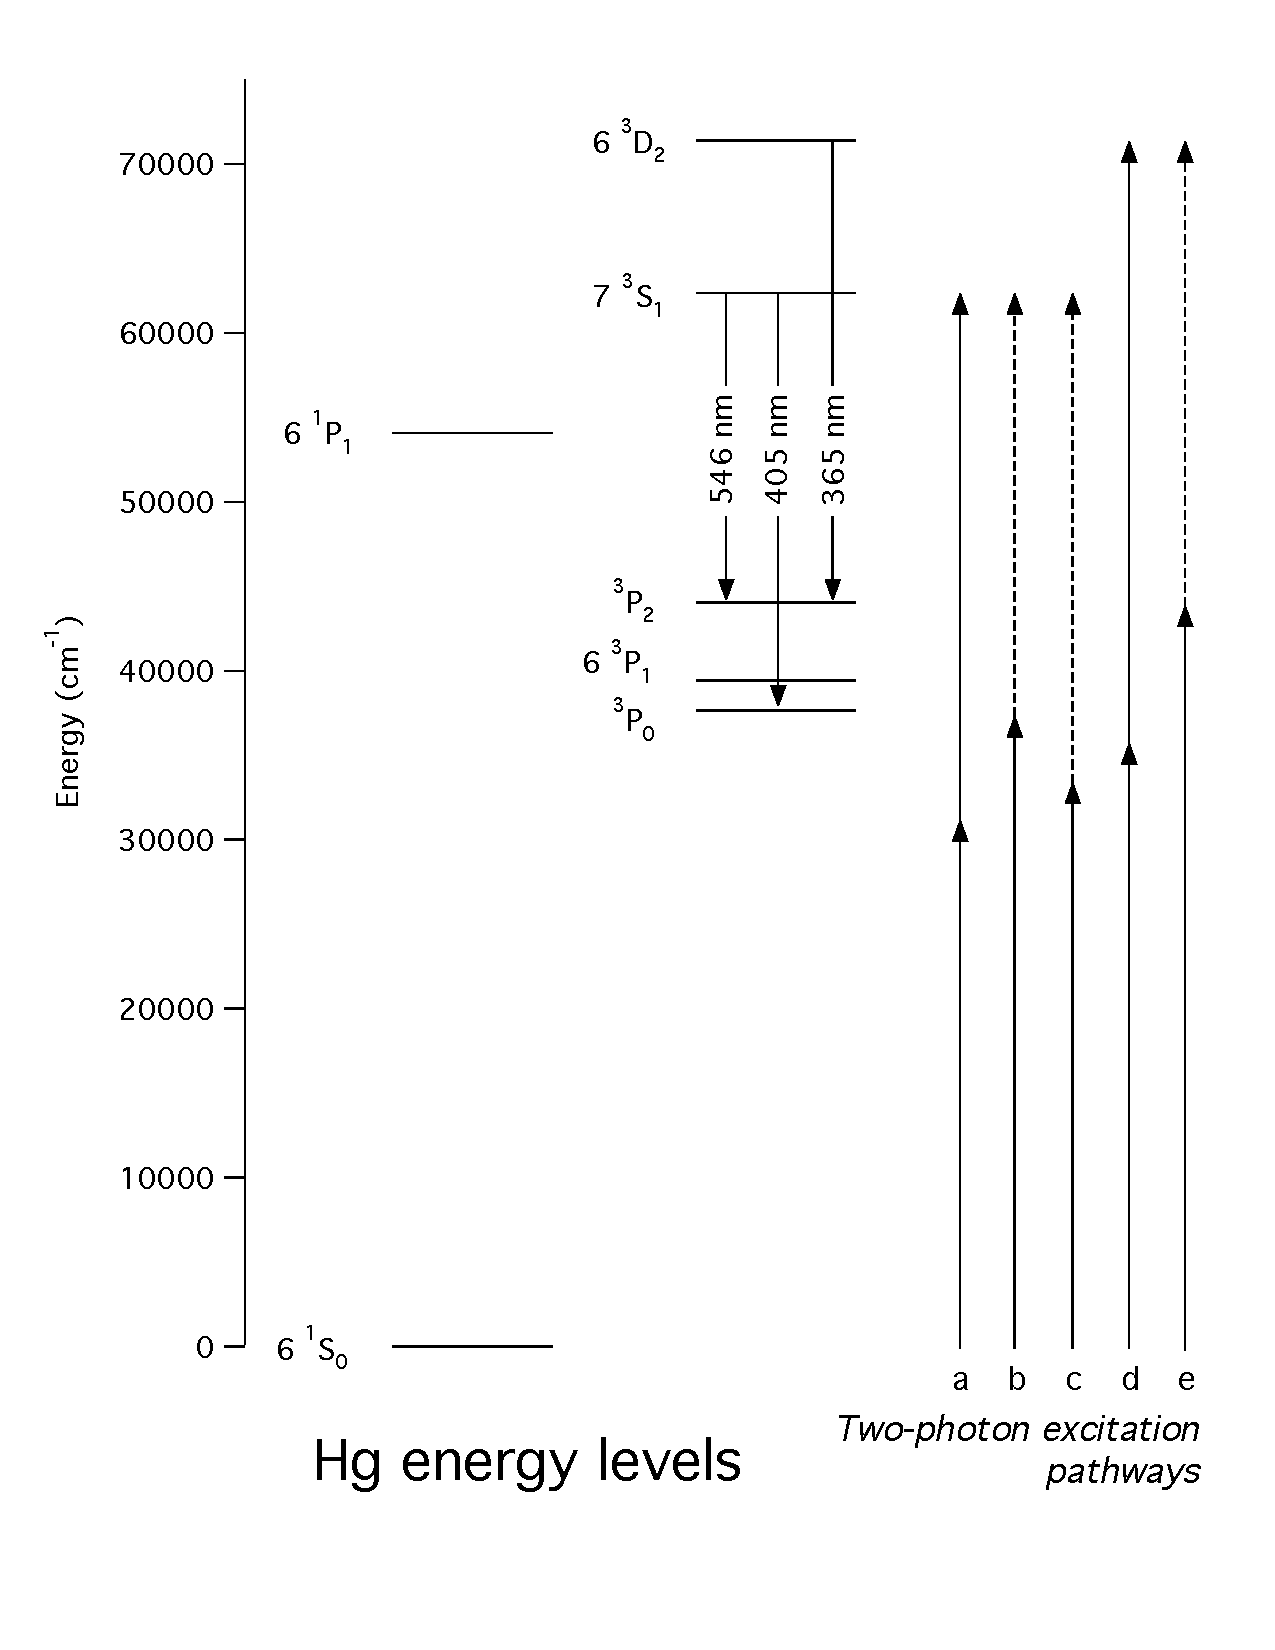
\includegraphics[height=8in,trim=4mm 0 0 0]{Hg-opticalpumpingschemes.pdf}
\end{figure}

% \begin{figure}
%   \caption{...}
%   \label{fig:tpa-prob}
% \end{figure}

The calculated transition probabilites for each scheme are displayed
in Figure \TODO{fig:hg-tpa-prob}.  The one color, two-photon
transition to the $6 \; ^3D_2$ level, item (d), has the greatest
transition probability among all the two-photon schemes considered.
The two-color transition to $6 \; ^3D_2$, item (e), is an order of
magnitude weaker.  The two color two-photon excitation schemes to the
$7 \; ^3S_1$ level, items (b) and (c), are an order of magnitude
weaker yet, and the one-color two-photon excitation to $7 \; ^3S_1$,
item (a), is forbidden entirely.

One color TPA to $7 \; ^3S_1$, is rigorously forbidden, due to
interference between the quantum mechanical pathways leading from the
initial to final state.  Figure \TODO{fig:hg-forbidden} shows the
possible pathways, and their phases according to Formula
\ref{eq:tpa-prob}.

The 

\section{Theory: A collision model for electronic excitation transfer}

Interest in the process of mercury photosensitization has led to the
study of the reaction of Hg $6 \; ^3P_1$ with many species
\cite{duval91, ohmori96}.

We base or mercury model on a collisional energy transfer model
originally developed for the Xe + \ce{N2} system by Ottinger and
Aquilanti \cite{aquilanti90, aquilanti94}.

Metastable xenon in the $^3P_2$ state transfers selectively into the
v'=5 level of \ce{N2}*($B\; ^3\Pi_g$) \cite{krumpelmann87,
  krumpelmann88, ottinger95b, aardema94}.  The process proceeds with
an absolute cross section of 6.5 $\AA$ \cite{bohle89}.

The angular momentum coupling rules for $P$-state atom collisions are
detailed by Aquilanti and coworkers \cite{aquilanti80a, aquilanti80b}.
The formalism is based on the idea of collisional Hund's cases,
explained by Nikitin and Zare \cite{nikitin94}.

The interaction potentials for $6 \; ^3P_0$ and $6 \; ^3P_2$ may be
estimated from those of the $6 \; ^3P_1$ state.  Having potential
surfaces in the collisional Hund's case (c) basis, the isotropic and
anisotropic parts of the interaction potentials may be determined
\cite{aquilanti89}.


\section{Experiments: \ce{Xe}* + \ce{N2}}

Two-photon excitation of xenon atoms followed by spontaneous
fluorescence is more commonly used to populate excited states \cite{alekseev96}.

The velocity distribution in a molecular beam is
\begin{equation}
  P(v) = v^3 \exp 
  \left [
    -\frac{m(v-u(x))^2}{2RT(x)}
  \right ],
\end{equation}
where $T(x)$ and $u(x)$ are the instantaneous temperature and flow
velocity in the beam \cite{morse96}.

\begin{figure}
  \caption{Potential energy curves and vibrational levels of the three
    ``lowest'' energy triplet electronic states of nitrogen, \ce{N2}.
    The $A$ state is metastable, with a fluorescence lifetime in the
    hundreds of microseconds.  Molecules in the $W$ state decay slowly
    to the near-degenerate $B$ electronic state via the emission of IR
    fluorescence.  The fluorescence lifetime for $B \rightarrow A$
    emission is several \microsec. It is this 400$-$500 nm
    fluorescence that we measure to observe the preparation of
    metastable \ce{N2}.  Also shown in the figure is the energy of the
    xenon $^3P_2$ state, which is known to populate the v'=5 level of
    the nitrogen $B$ state in gas-phase collisions
    \cite{krumpelmann87}.  Less is known about electronic energy
    transfer from Xe into the $W$ state of nitrogen, however, the
    ultimate decay route is unchanged in any case.  The figure is
    adapted from Reference \cite{krumpelmann-thesis}.}
  \label{fig:n2curves}
  \centering
  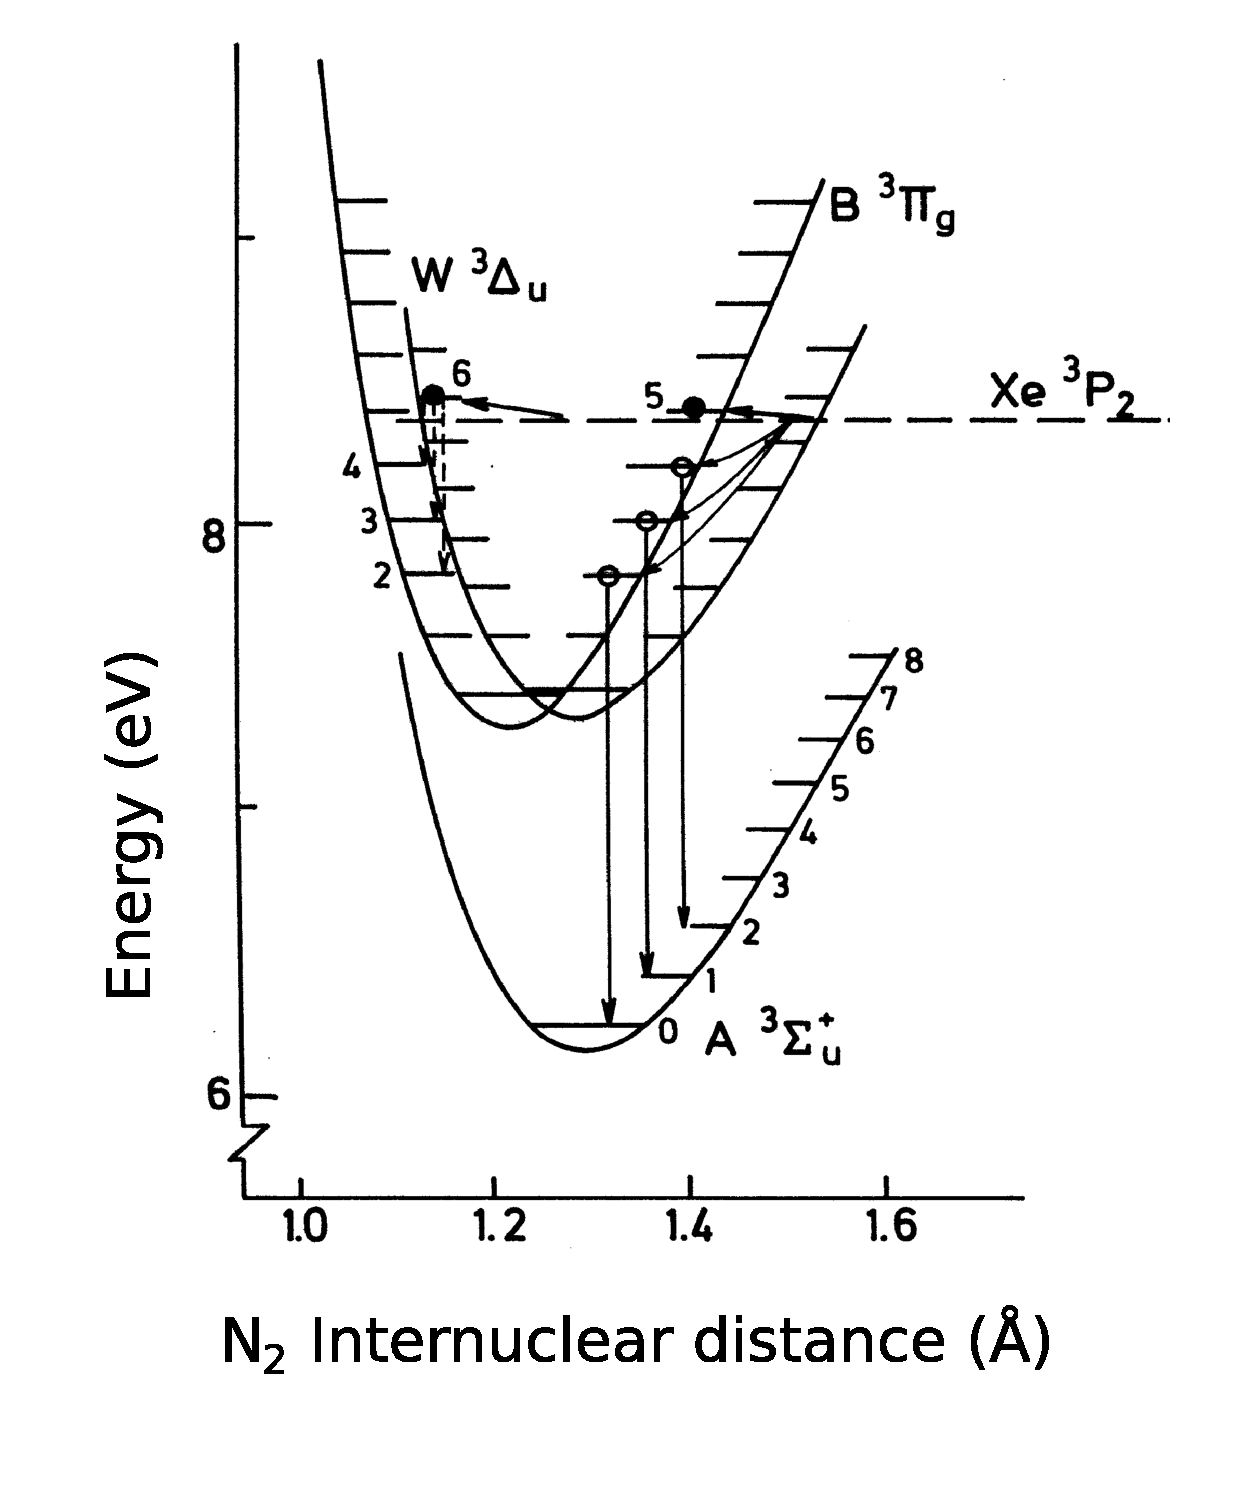
\includegraphics[width=5in]{n2curves.pdf}
\end{figure}

\begin{figure}
  \caption{Laser-Induced Fluorescence (LIF) spectrum of the one color,
    two photon transition \ce{Xe} $6\;^3D_2 \leftarrow \leftarrow
    6\;^1S_0$, recorded under static cell conditions.  The LIF signal
    results from spontaneous emission to the metastable $6\;^3P_2$
    state at 823 nm.}
  \label{fig:xe3d2-cell}
  \centering
  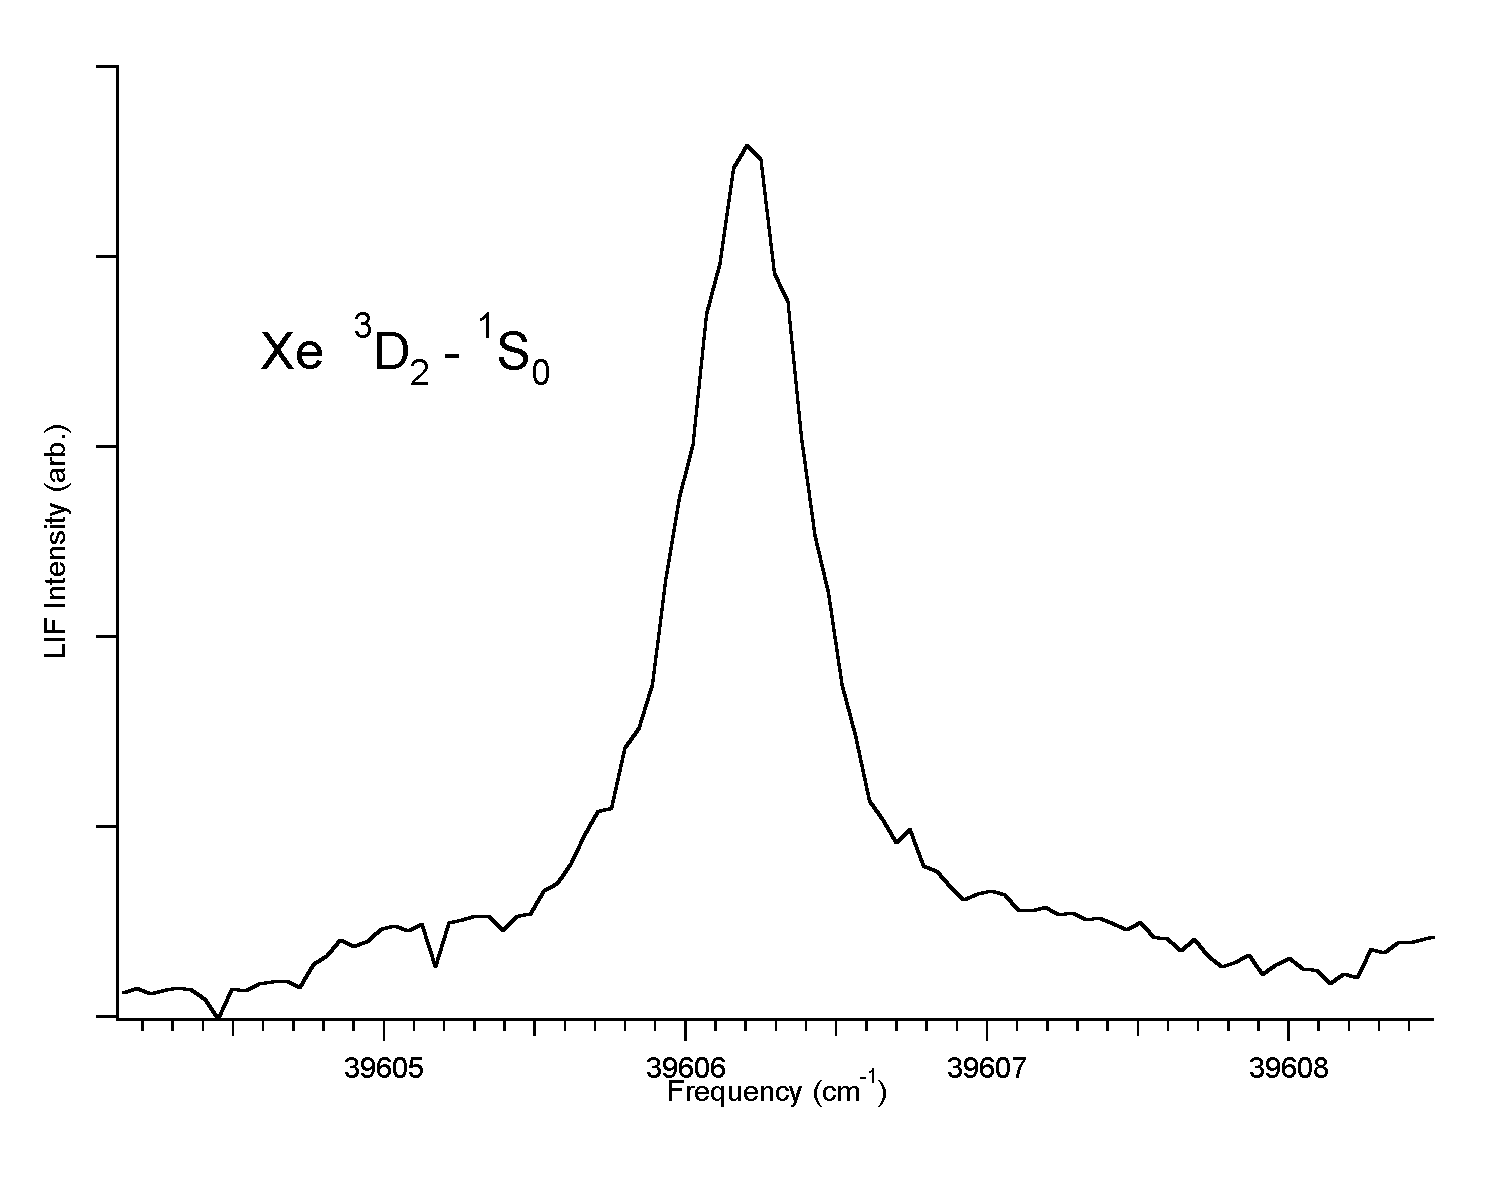
\includegraphics[width=6in]{Xe3D2-cell.pdf}
\end{figure}

\begin{figure}
  \caption{Time dependence of \ce{N2} $B \rightarrow A$ emission,
    induced by collisions with metastable Xe* ($^3P_2$).  The static
    cell contained a 50:50 mixture of Xe and \ce{N2}, at a total
    pressure of 210 mTorr.  Metastable Xe* ($^3P_2$) was populated by
    spontaneous emission, following the $6\;^3D_2 \leftarrow
    \leftarrow 6\;^1S_0$ two-photon transition.}
  \label{fig:xen2-firstlight}
  \centering
  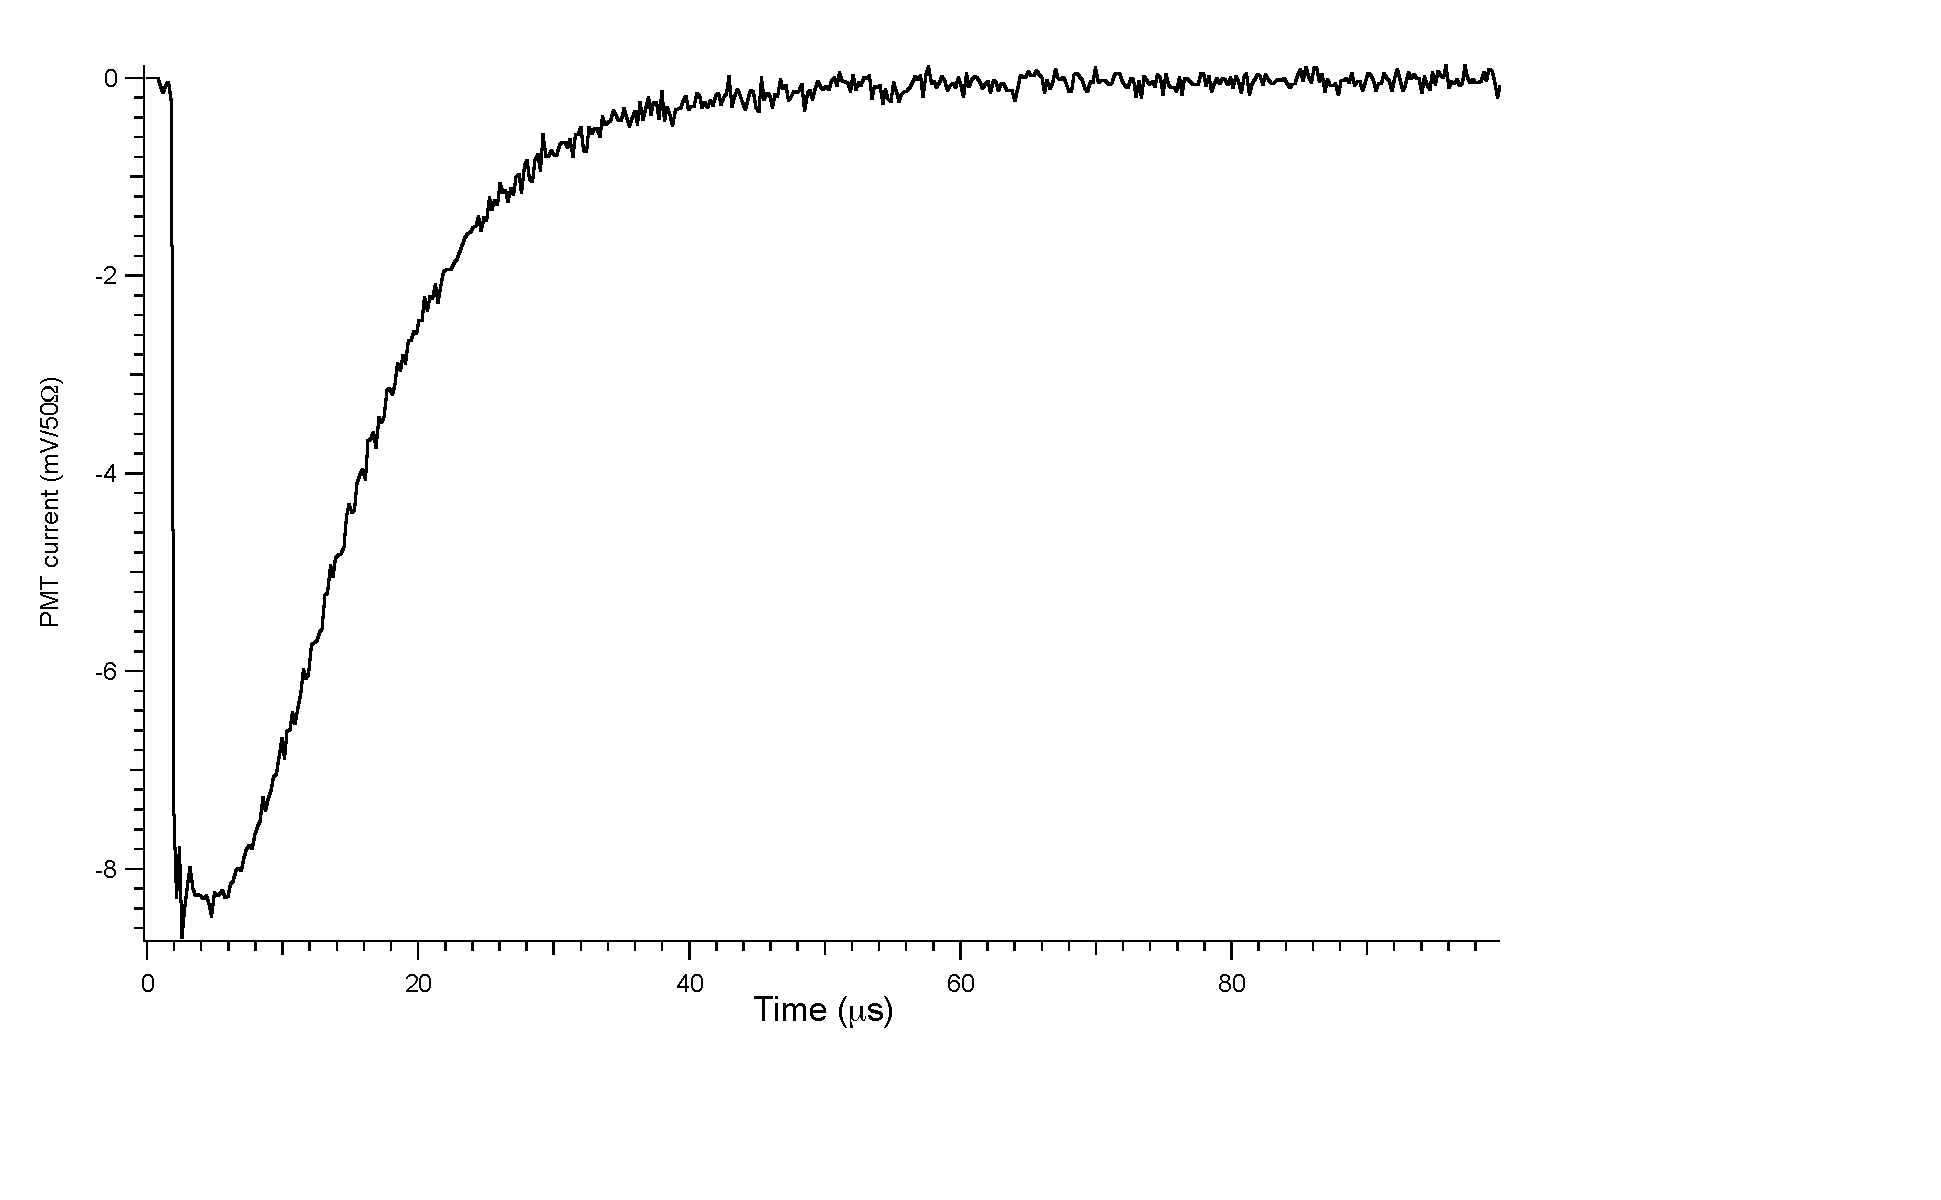
\includegraphics[width=7in,trim=2cm 0 1in 0]{XeN2-firstlight.pdf}
\end{figure}

\begin{figure}
  \caption{(Top) Laser-Induced Fluorescence (LIF) spectrum of the one
    color, two photon transition \ce{Xe} $6\;^3D_2 \leftarrow
    \leftarrow 6\;^1S_0$, recorded in a supersonic expansion.
    (Bottom) Time dependence of \ce{Xe} $6\;^3D_2 \rightarrow
    6\;^3P_2$ emission (solid trace), compared to a magnified signal
    resulting from scattered laser light (dashed trace). The
    fluorescence signal results from spontaneous emission to the
    metastable $6\;^3P_2$ state at 823 nm ($\tau = 28$ ns).
    \TODO{Change top plot to LIF intensity.}}
  \label{fig:xe-beam}
  \centering
  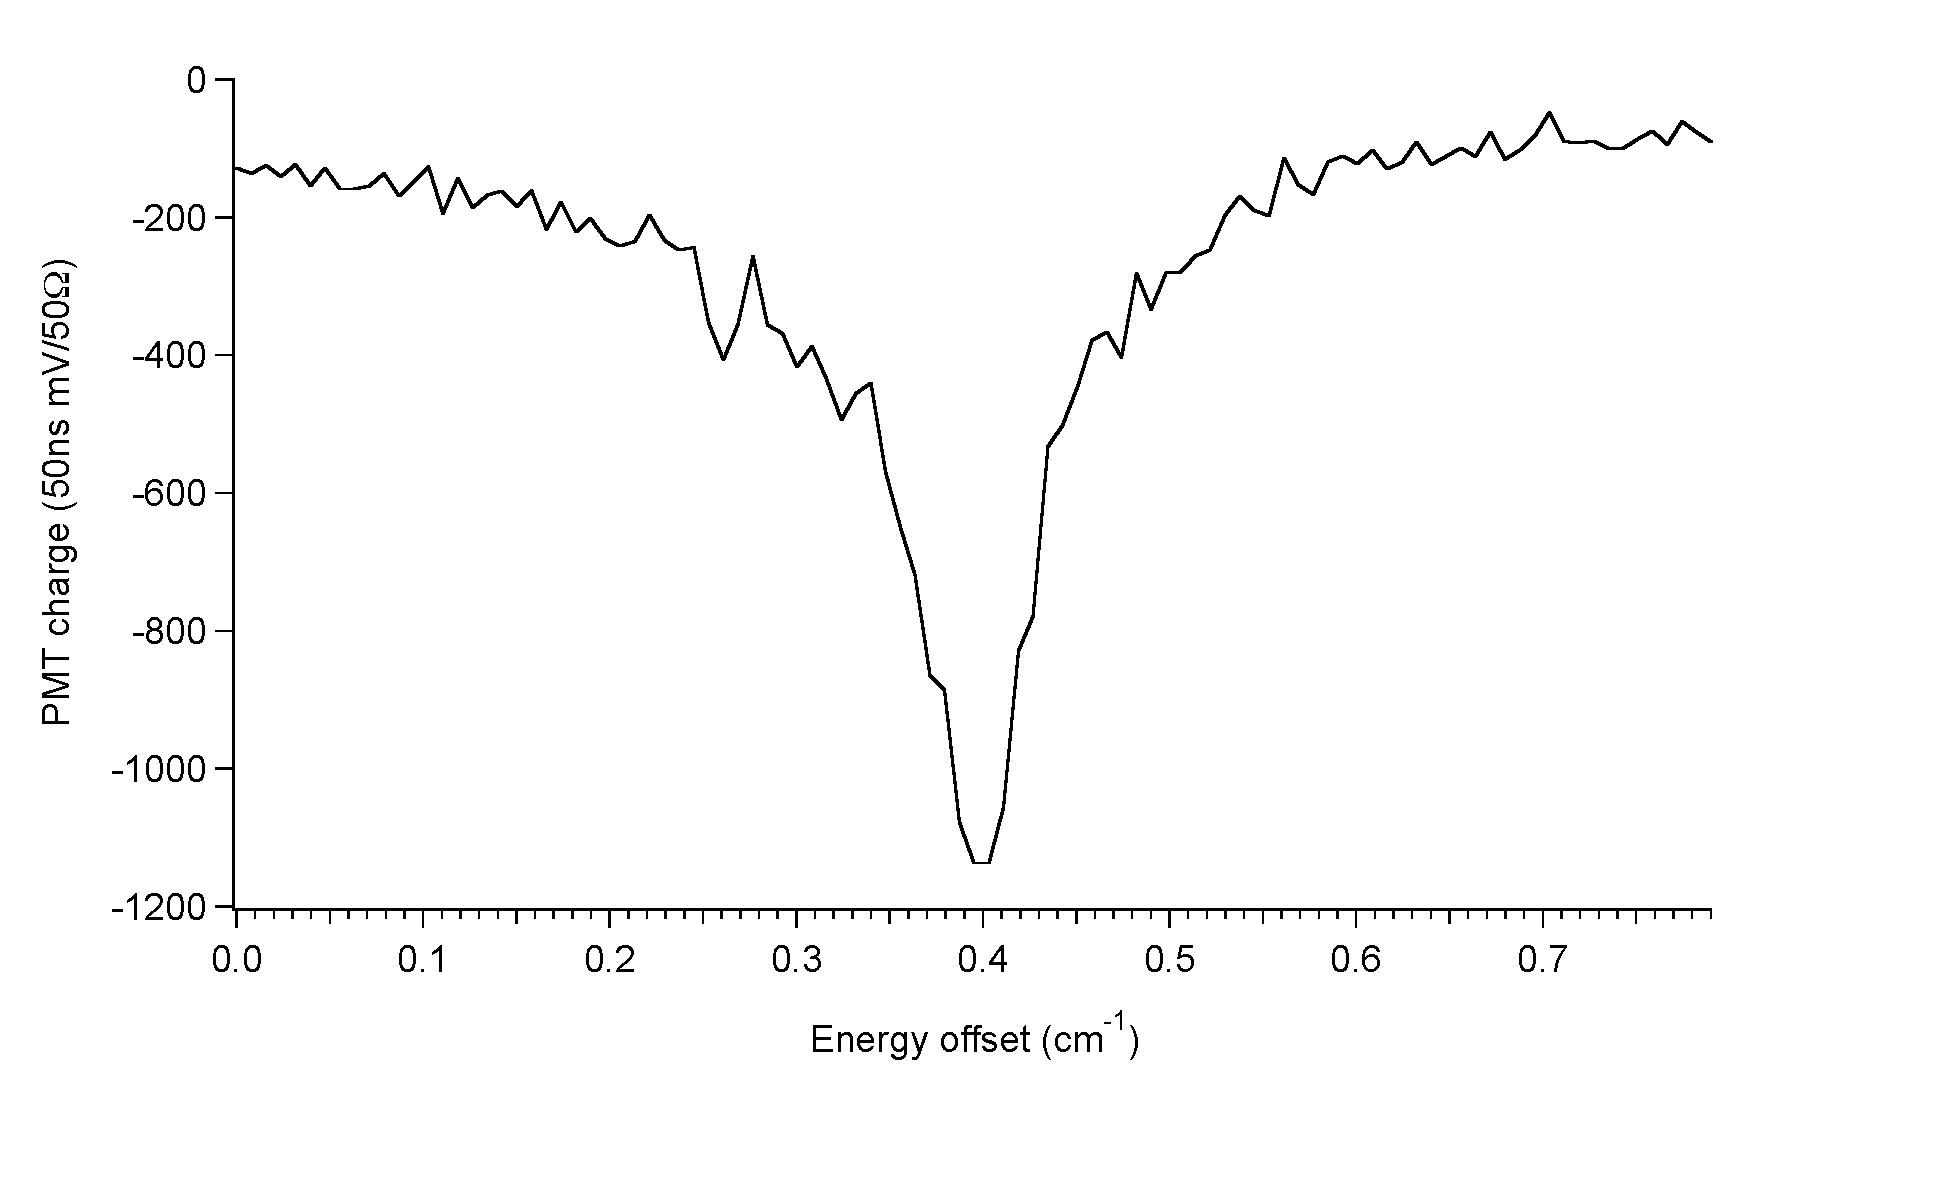
\includegraphics[width=6in]{Xe-beamlif-060406.pdf}
  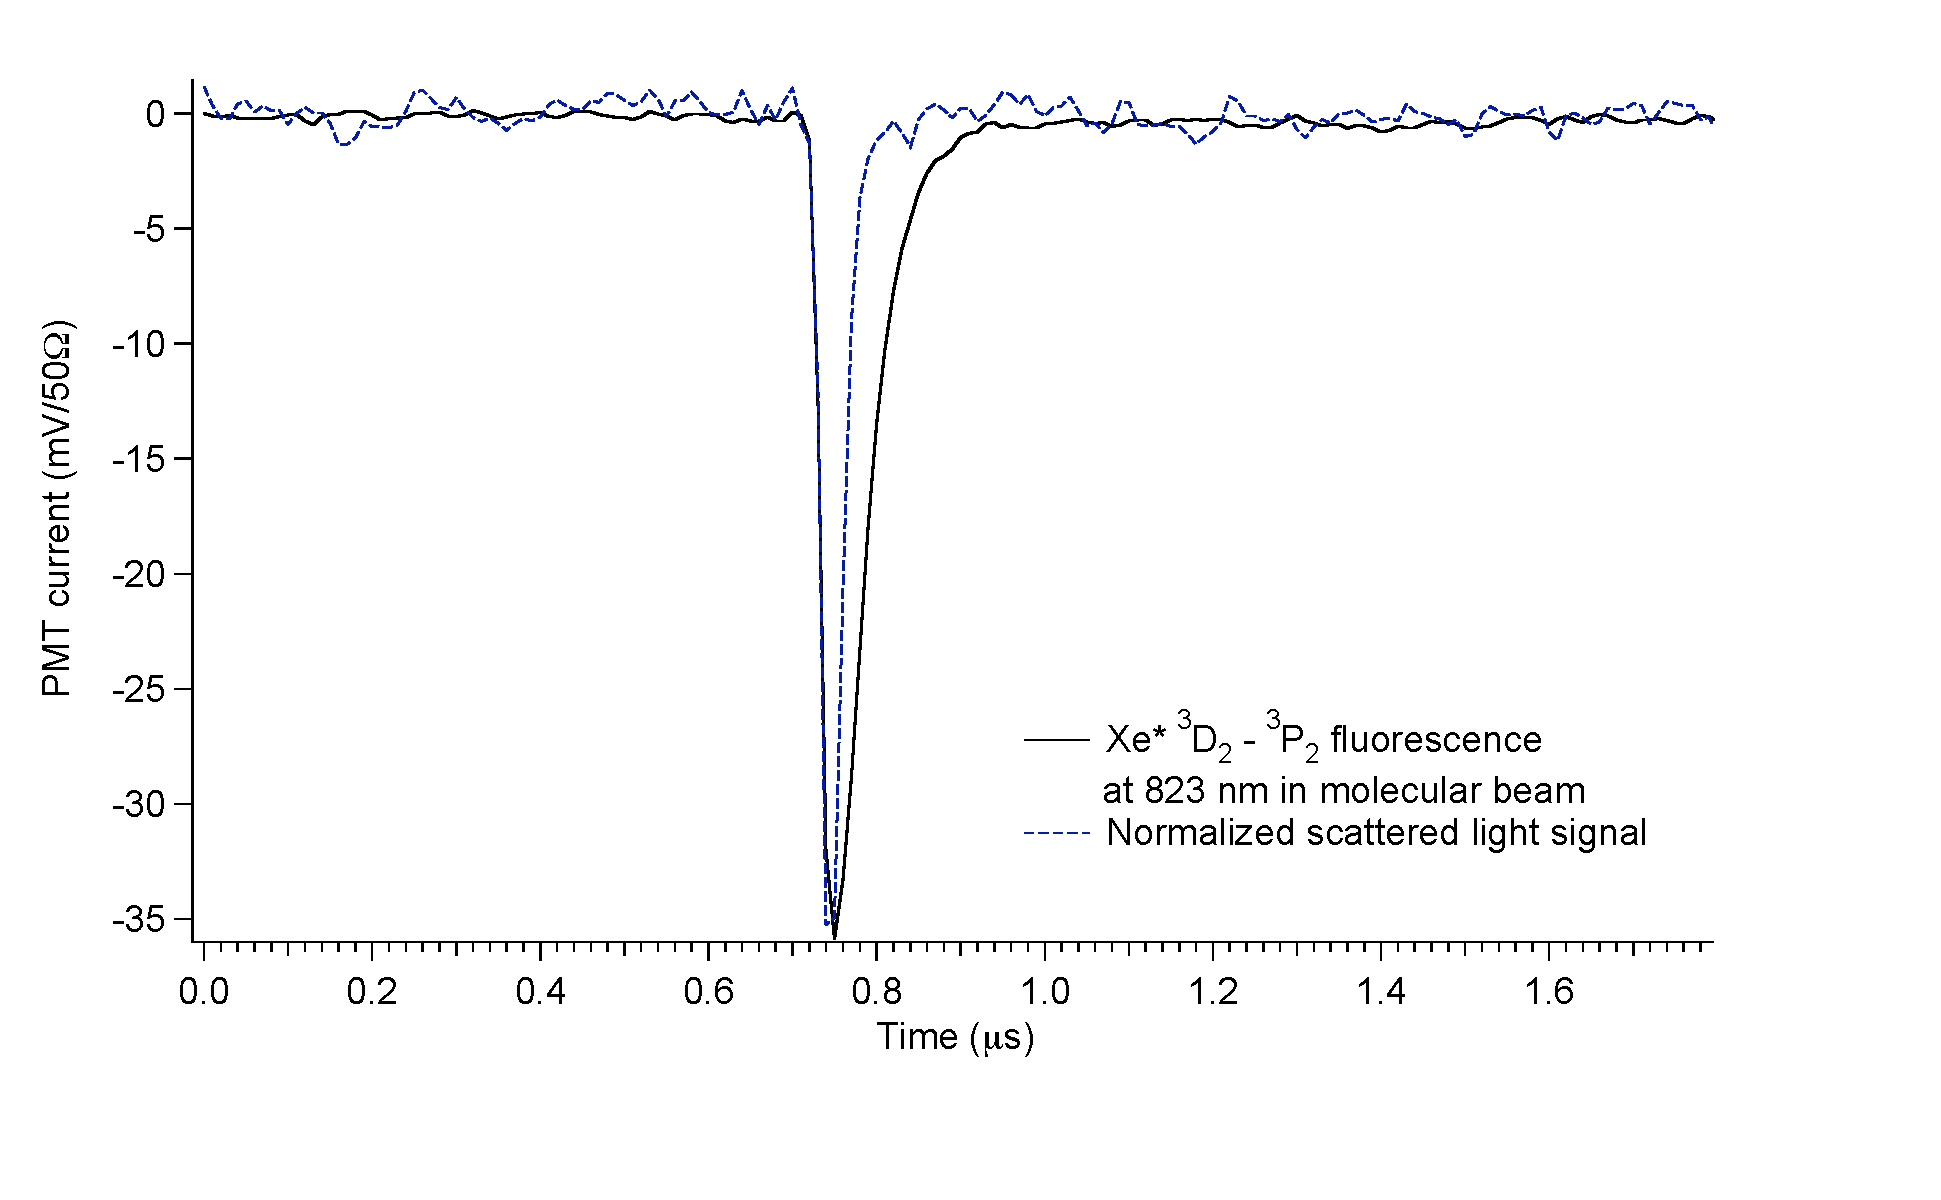
\includegraphics[width=6in]{Xe-beamtrc-060406.pdf}
\end{figure}

\begin{figure}
  \caption{Time dependence of \ce{Xe} $6\;^3D_2 \rightarrow 6\;^3P_2$
    (top plot) and \ce{N2} $B \rightarrow A$ (bottom plot) emission,
    following the two-photon excitation of Xe ($^3D_2$) in a
    supersonic expansion.  The xenon and nitrogen emission signals
    occur on vastly different timescales.  Xenon fluorescence (823 nm,
    $\tau=28$ ns) is emitted when the optically excited state decays
    spontaneously to the metastable $6\;^3P_2$ state.  Nitrogen
    molecules are electronically excited during the expansion process
    in collisions with metastable xenon atoms.  Near-resonant
    vibrational levels of the nitrogen $B$ state decay spontaneously
    to the metastable $A$ state ($\tau=20$ \microsec), accompanied by
    fluorescence in the visible region of the spectrum. \TODO{Change
      voltage to current.}}
  \label{fig:xen2-traces}
  \centering
  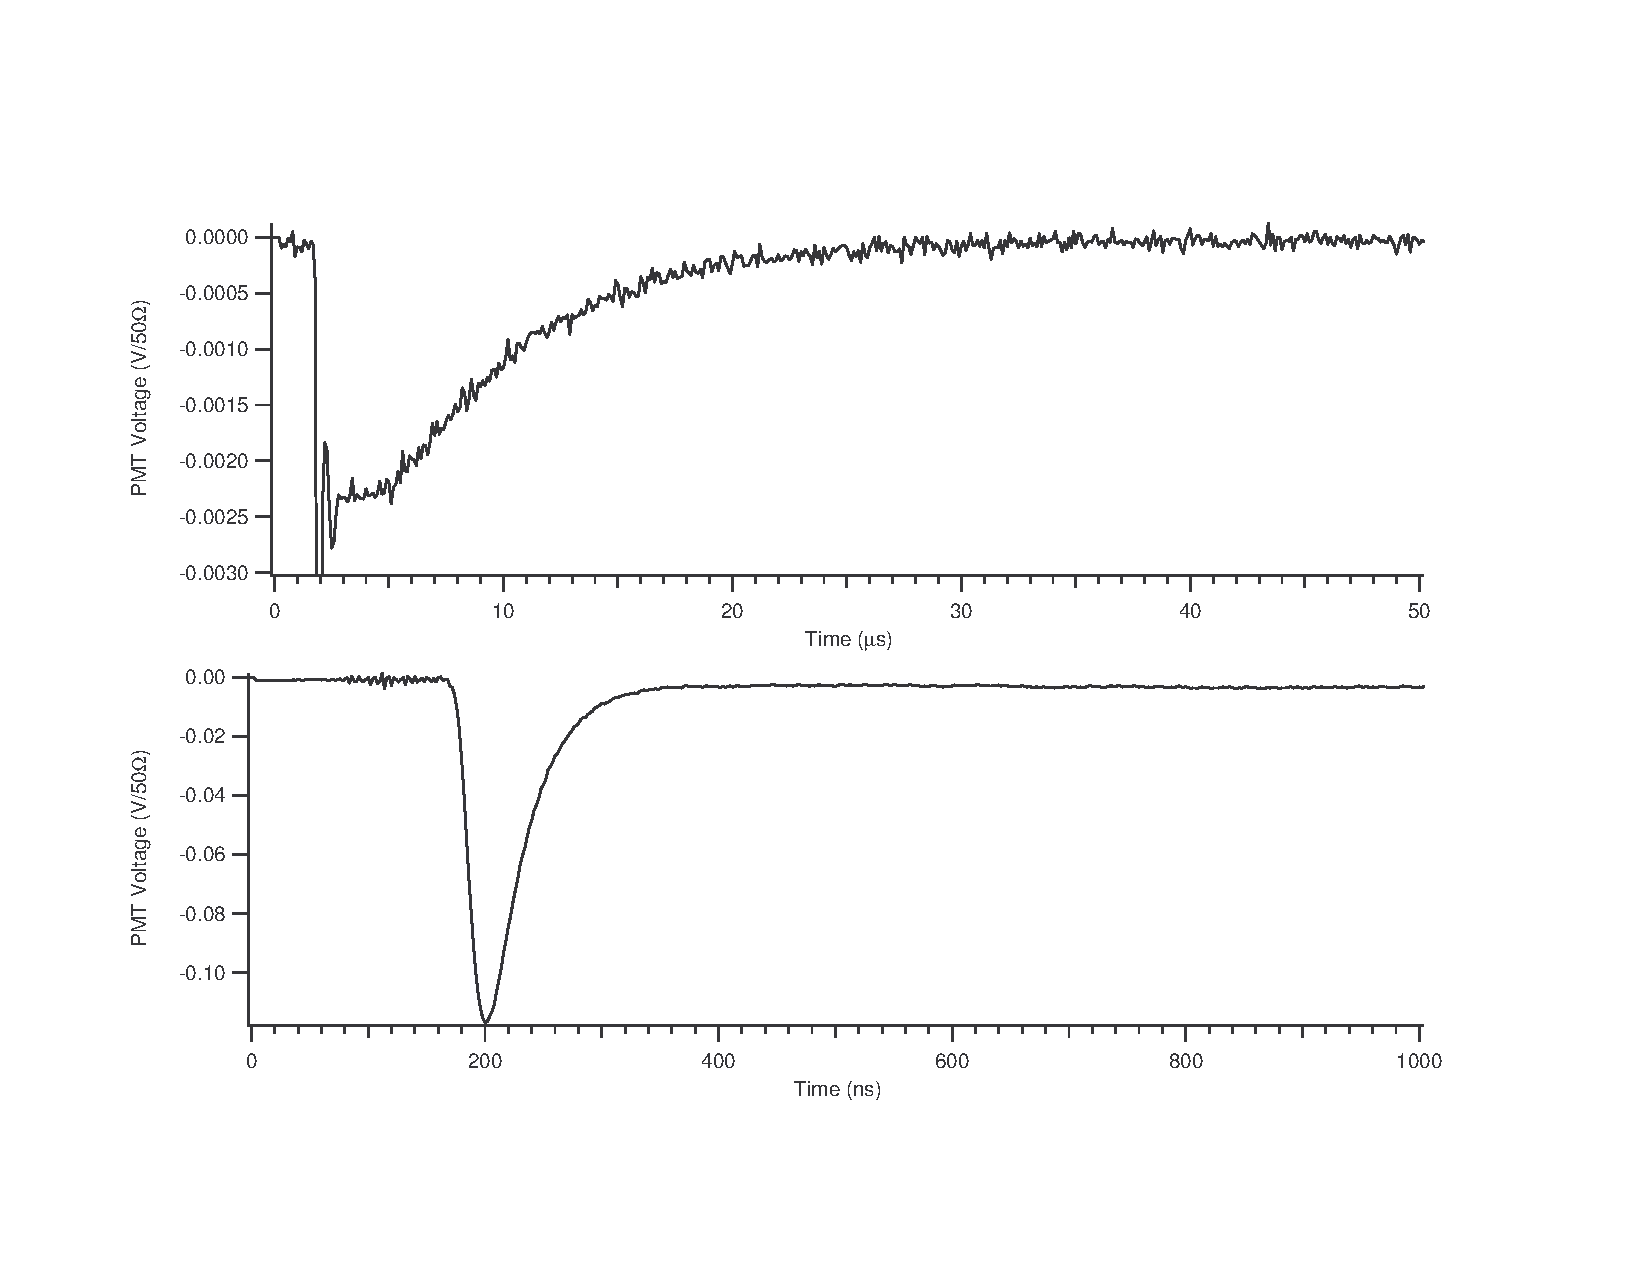
\includegraphics[width=7.7in,angle=90,trim=0 0 1in 1cm ]{XeN2-traces.pdf}
\end{figure}



\section{Experiments: \ce{Hg}* + \ce{C2H2}}

Continuous beam sources of mercury $6 \; ^3P_0$ are reported in the
literature \cite{haberman75, obi83}.  Nitrogen backing gas is first
bubbled through a mercury oven before expanding from a nozzle with an
embedded resonance lamp.

We also attempted to populate the $^3P_0$ level of mercury by
collisional relaxation with \ce{N2} molecules.  Nitrogen is known to
efficiently quench Hg*($6 \; ^3P_1$) to Hg*($6 \; ^3P_0$), because the
intramultiplet energy difference is about the same as the vibrational
level spacing in \ce{N2} \cite{callear70, horiguchi71}.  Bras and
coworkers meaured the energy transfer dynamics of mercury in \ce{N2}
buffer gas, and determined that Hg($^3P_0$) may be efficiently
produced by the decay process Hg($7 \; ^1S_0$) $\rightarrow$ Hg($6 \;
^3P_1$) $\rightarrow$ Hg($6 \; ^3P_0$) \cite{bras93}.



\begin{figure}
  \caption{Laser-Induced Fluorescence (LIF) spectrum of the one color,
    two photon transition \ce{Hg} $6\;^3D_2 \leftarrow \leftarrow
    6\;^1S_0$, recorded under static cell conditions.  The LIF signal
    results from spontaneous emission to the metastable $6\;^3P_2$
    state at 365 nm.}
  \label{fig:hg3d2-cell}
  \centering
  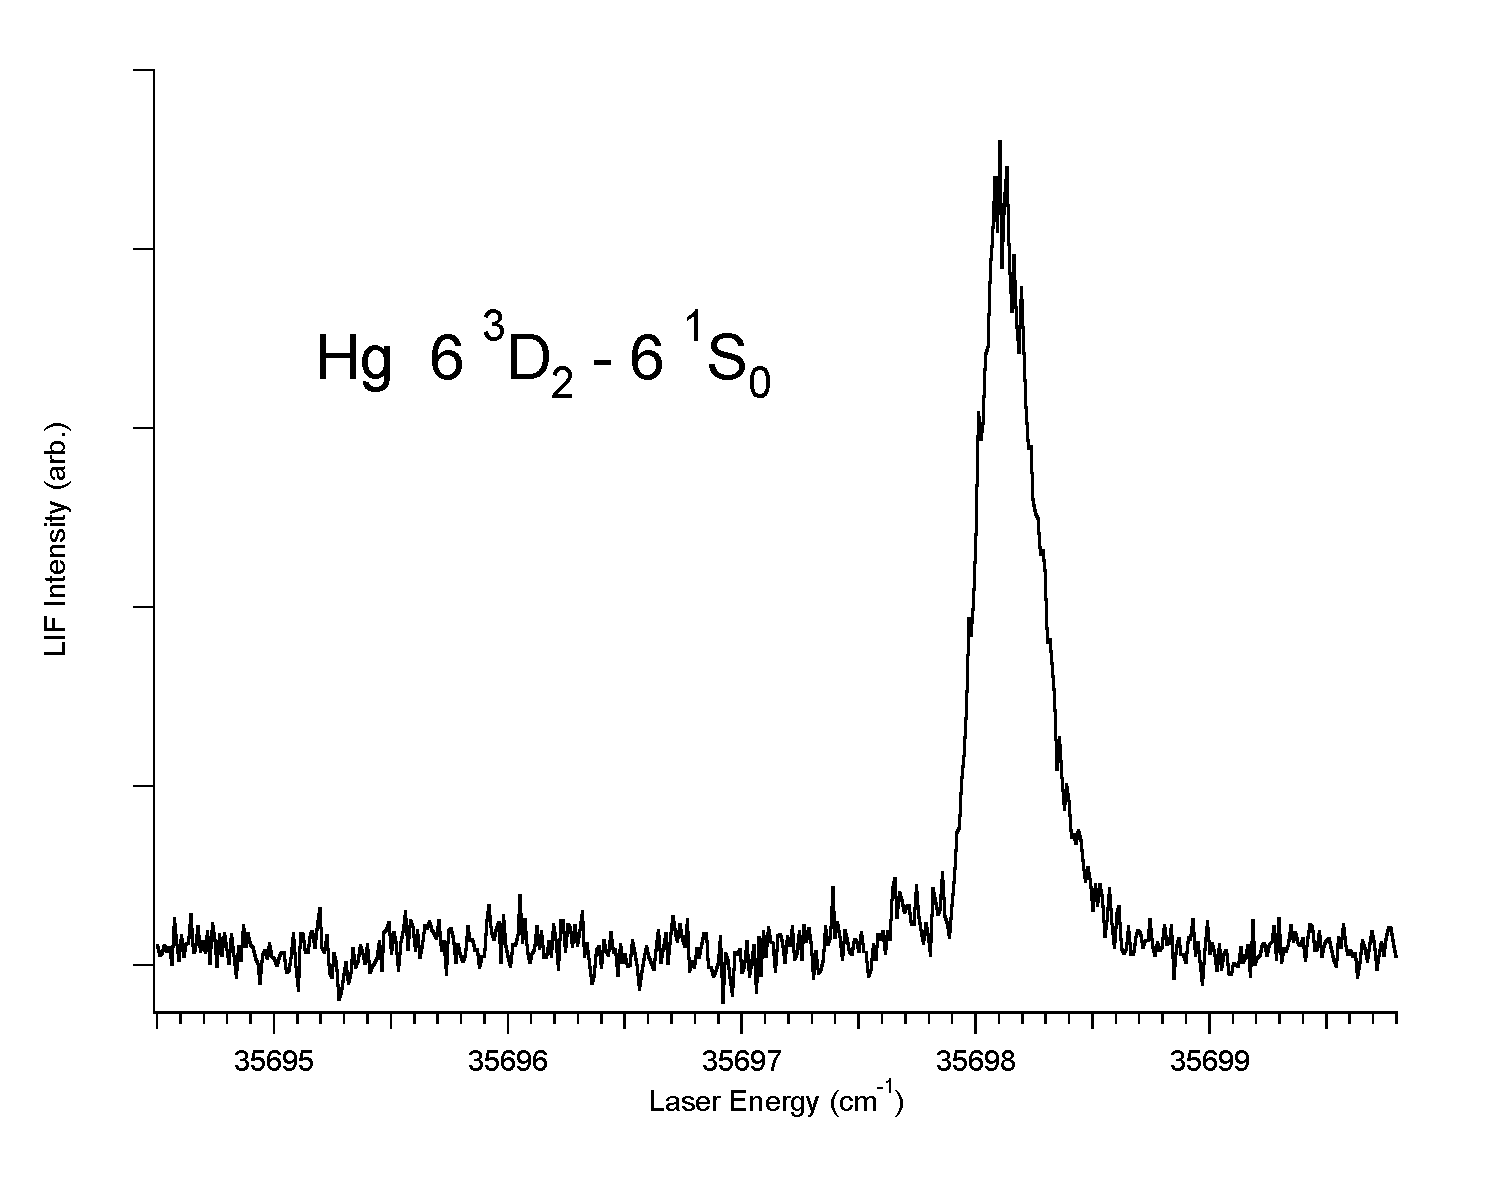
\includegraphics[width=6in]{Hg3D2-cell.pdf}
\end{figure}

A new pulsed valve was designed by Wilton Virgo to meet our demands
for heated mercury.  A diagram of the ``Bern Valve'' is shown in
Figure \ref{fig:bern-diagram}.

\begin{figure}
  \caption{Diagram of the heated pulsed valve developed for
    experiments with mercury.  The ``Bern Valve'' can be safely heated
    to 250\degrees\ C.  A small vial of mercury is housed in the
    heated region on the right of the diagram, close to the nozzle
    orifice (far right).}
  \label{fig:bern-diagram}
  \centering
  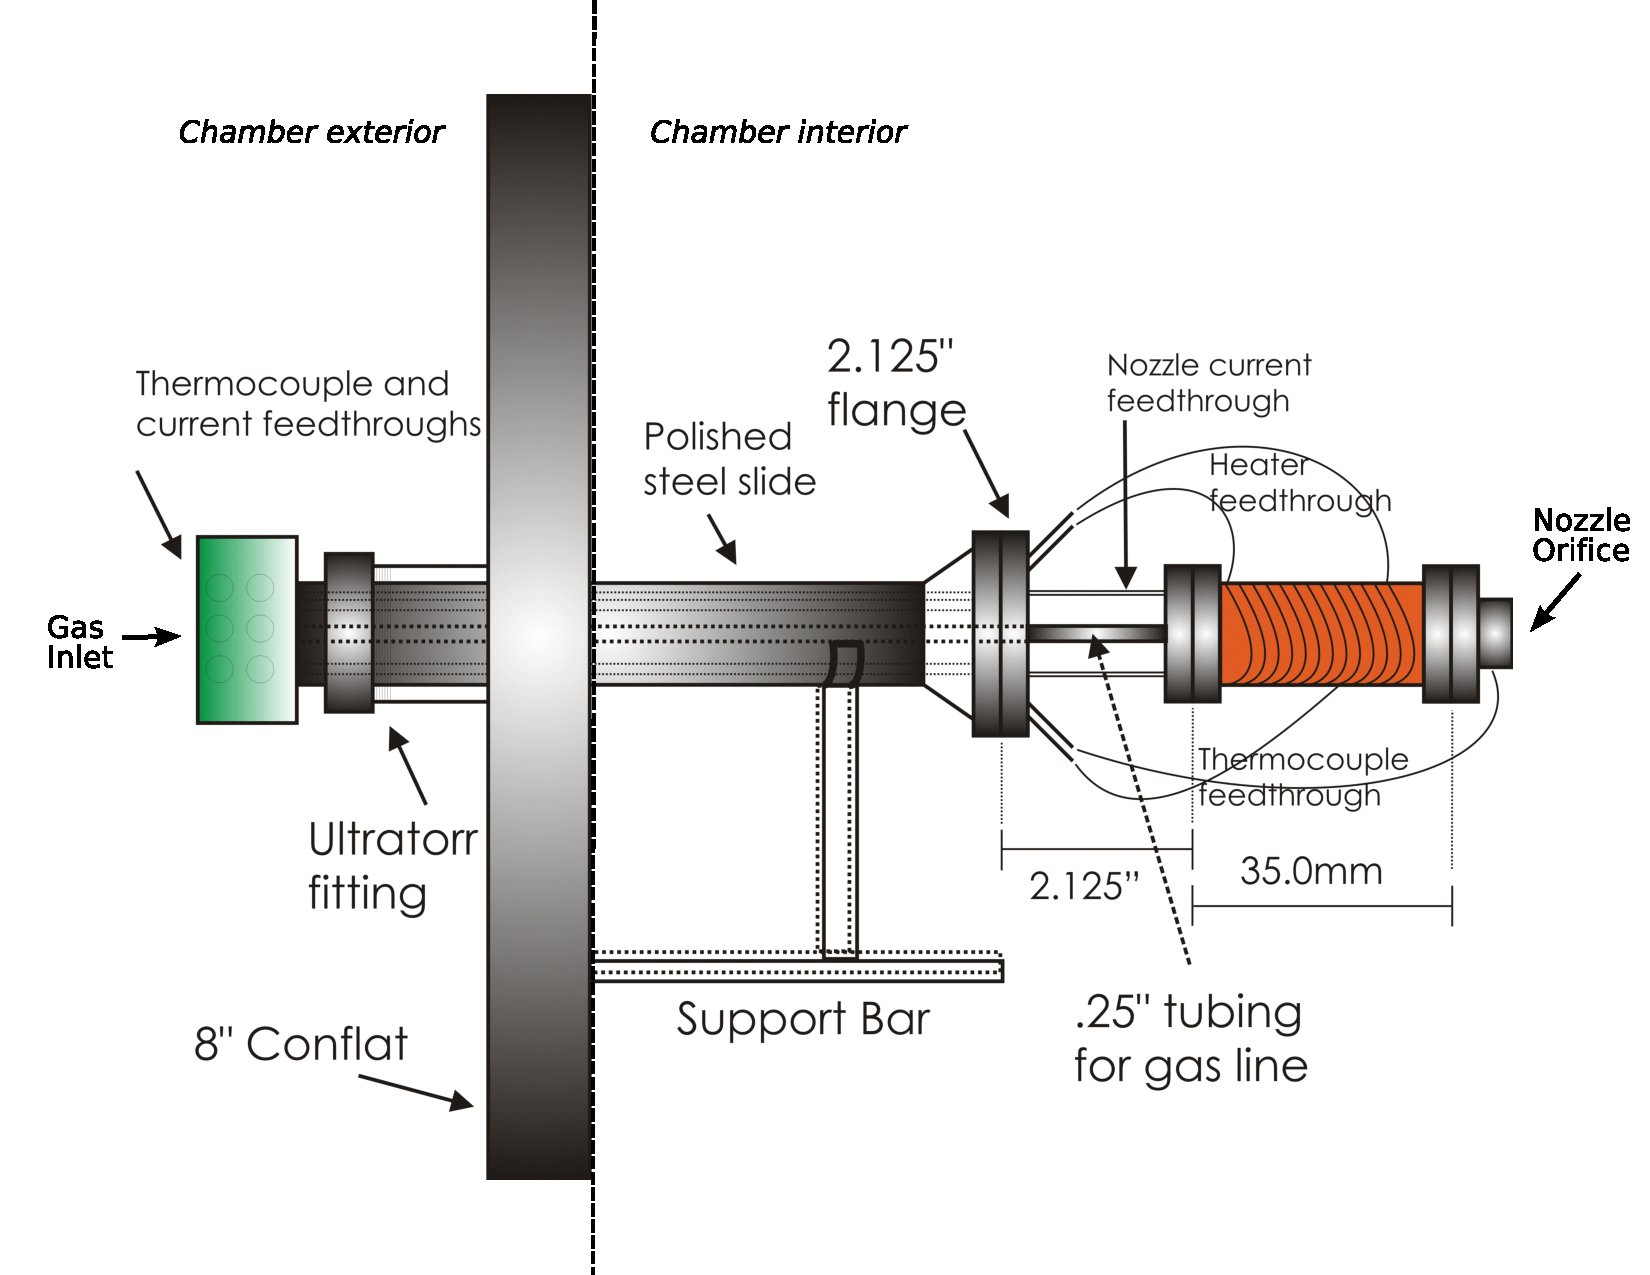
\includegraphics[width=6in]{bern-diagram.pdf}
\end{figure}



% \TODO{Figure: Direct excitation to Hg*($^3P_2$). (See p.47 of
%   11/2007--1/2008 notebook.)}  
Direct excitation to the $6 \; ^3P_2$ was attempted as a method for
triplet formation.  This transition, while forbidden in the solitary
molecule, is made allowed in collision complexes with a variety of
gases \cite{kurosawa98, amano98}.  Also, we note that weak Hg*($6 \; ^3P_2$)
$\rightarrow$ Hg($6 \; ^1S_0$) emission was observed in pre-laser
experiments \cite{mrozowski45}.  Figure \ref{fig:hg-3p2-direct} shows
the TOF:SEELEM spectrum of mercury excited to directly to the $6 \;
^3P_2$ level.  The signal level is sufficiently low that it is checked
against a repeated experiment with the pulsed valve turned off, shown
for comparison in Figure \ref{fig:hg-3p2-direct-bg}.  While it is
clear that we do register a SEELEM signal from the direct excitation
of Hg*($6 \; ^3P_2$), we were not able to increase the gas density
enough at the excitation point to make this an efficient process for
the population of acetylene metastables.

\begin{figure}
  \caption{SEELEM time of flight (TOF) detection of metastable mercury
    produced via the direct excitation Hg*($6 \; ^3P_2$) $\leftarrow$
    Hg($6 \; ^1S_0$) at 44042.98 \rcm.  The pulsed valve was heated to
    250\degrees\ C to increase the number density of mercury.  The two
    traces are recorded in repeated experiments.}
\label{fig:hg-3p2-direct}
\centering
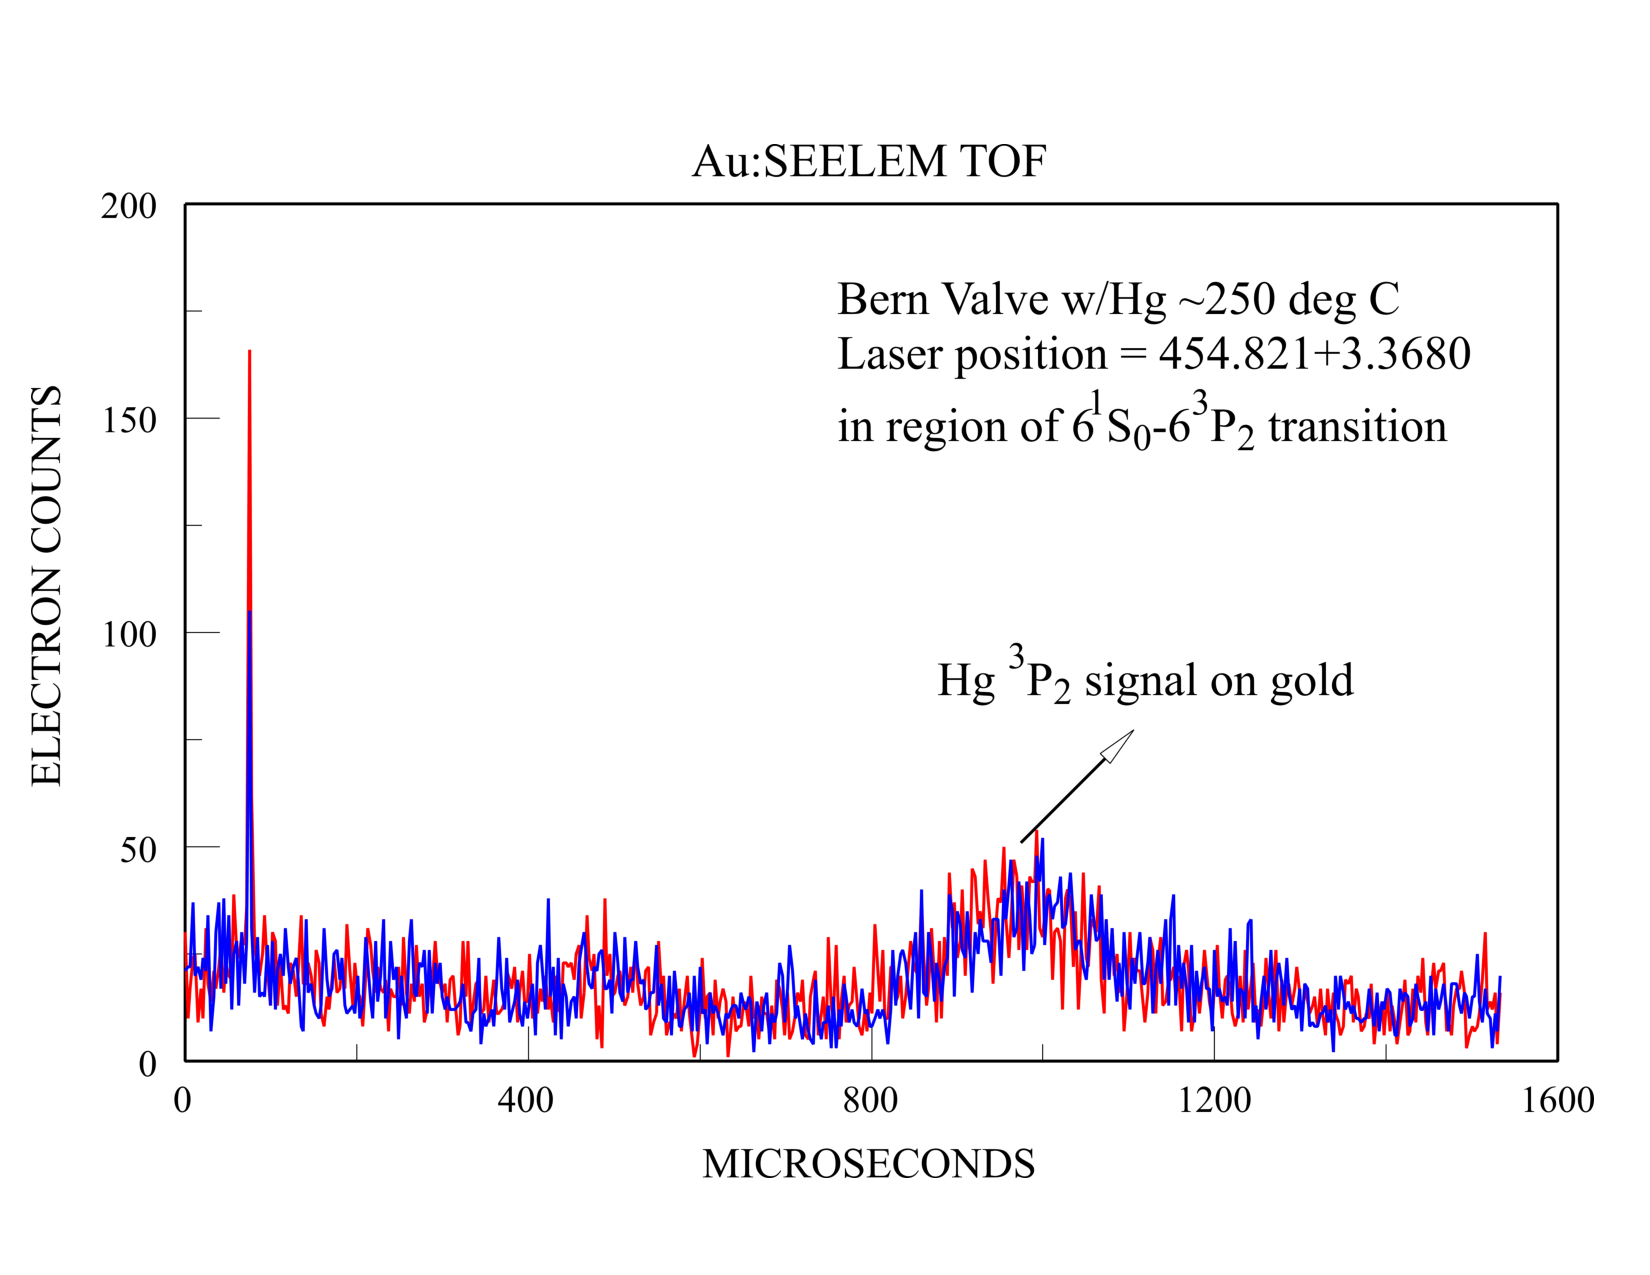
\includegraphics[width=8in,angle=90]{hg-3p2-direct.pdf}
\end{figure}

\begin{figure}
  \caption{Comparison of signal to background in the SEELEM time of
    flight (TOF) detection of metastable mercury produced via the
    direct excitation Hg*($6 \; ^3P_2$) $\leftarrow$ Hg($6 \; ^1S_0$)
    at 44042.98 \rcm.  The lighter trace is recorded with the pulsed
    valve on, and the black trace is recorded with the valve off.}
\label{fig:hg-3p2-direct-bg}
\centering
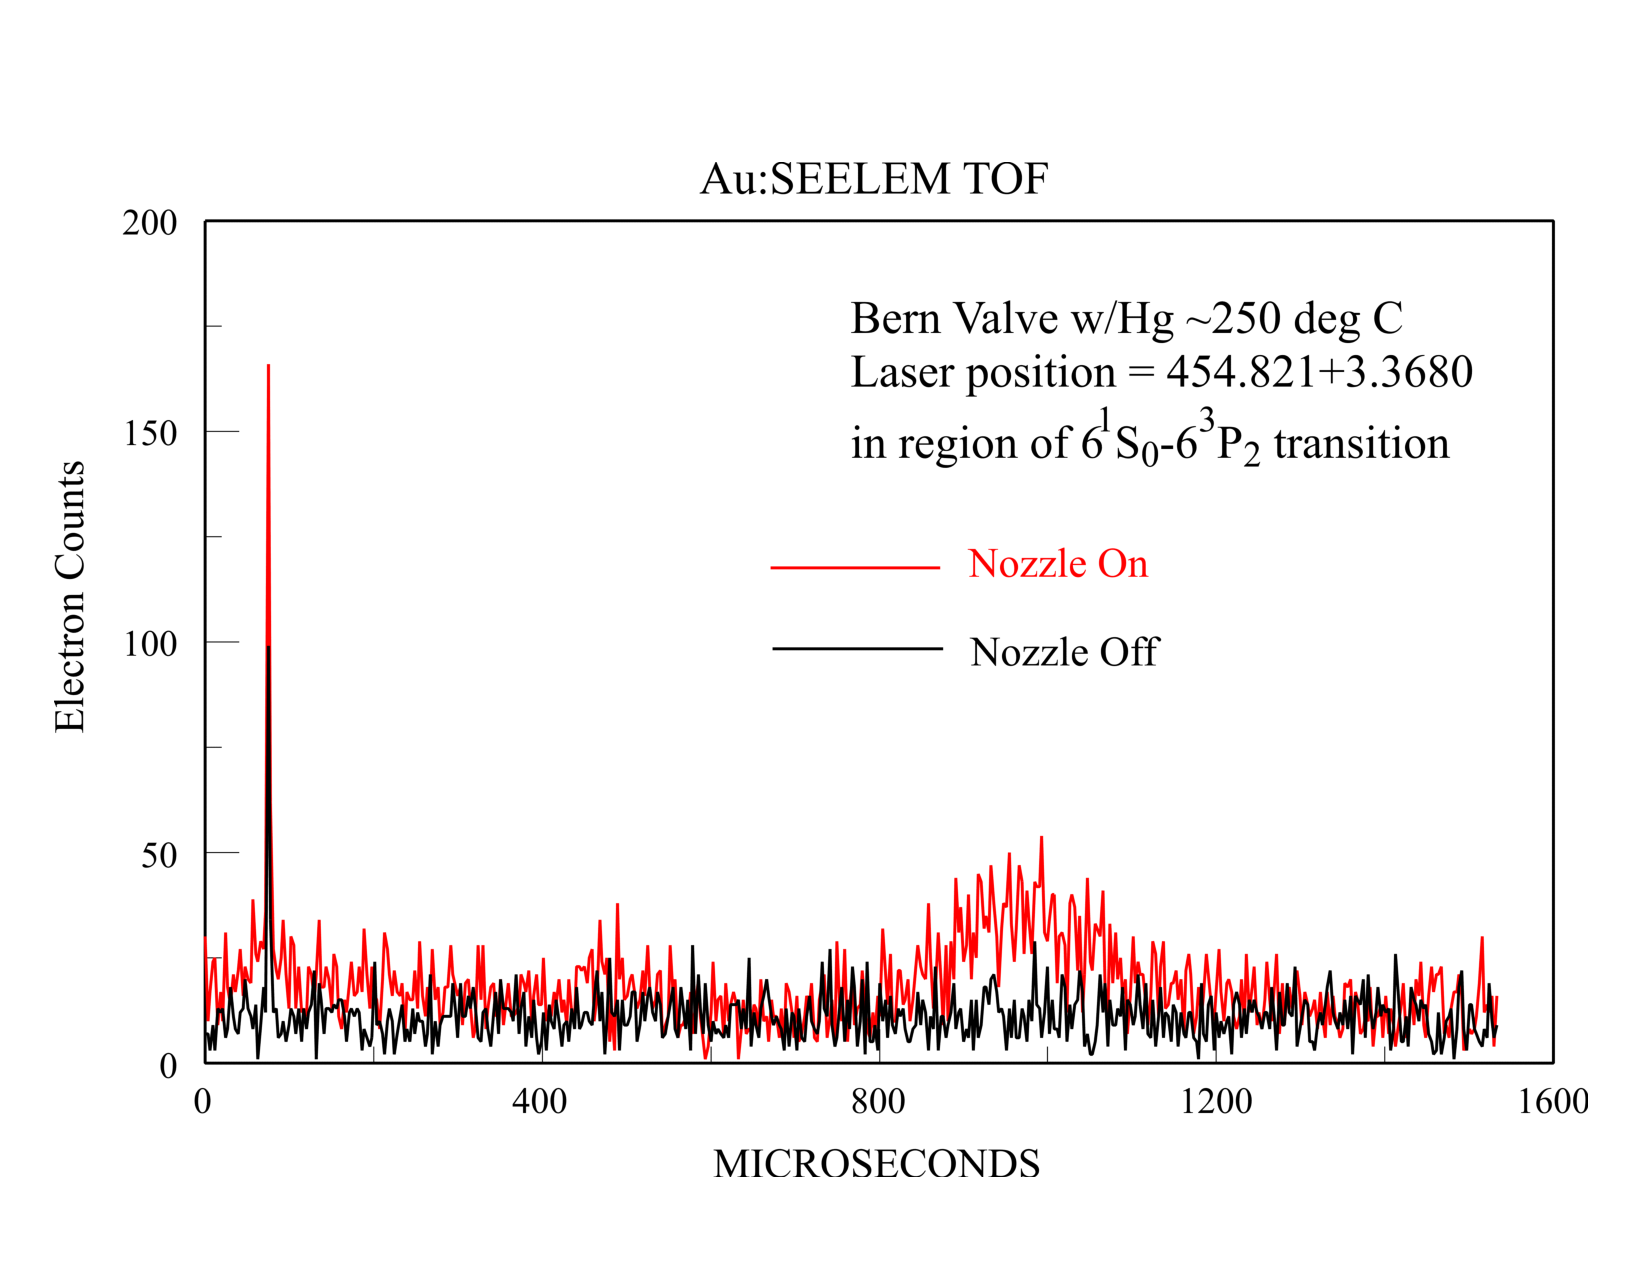
\includegraphics[width=8in,angle=90]{hg-3p2-direct-bg.pdf}
\end{figure}

The most efficient method we found for the population of mercury $6 \;
^3P_2$ was a simple, two step excitation to $7 \; ^3S_1$ via the $6 \;
^3P_1$ level.  Figure ??? shows the LIF spectrum of the $6 \; ^3P_1
\leftarrow 6\;^1S_0$ transition.  The hyperfine structure of the ???
and ??? isotope are apparent in the lineshape of the transition.

Methods are available to optically filter mercury resonance radiation
using mercury itself as the absorber \cite{vanzee89, senitzky74}.

\section{Conclusions}

An exciting experiment for the xenon-nitrogen system would be to study
the rotational and vibrational depenence of collision-induced reverse
intersystem crossing from the $a' \; ^1\Sigma_u^-$ state to the $B \;
^3\Pi_g$ state.  Xenon has been observed to facilitate this process,
although the rotational and vibrational dependence are uncertain
\cite{umemoto03a}.

\bibliography{master} 
\bibliographystyle{plain}
\end{document}